\chapter{Corrections to the cross sections}
\label{Sect:corr_cr_sect}

This chapter gives the description of the corrections to the extracted cross sections in the order they were applied.


\section{Filling kinematic cells with zero acceptance}
\label{Sect:empt_cells}

Due to blind areas in the geometrical coverage of the CLAS detector, some kinematic bins of the double-pion production phase-space turned out to have zero acceptance. In such bins, which are usually called empty cells, the cross section cannot be experimentally defined. For the studies, which aim at extracting fully-differential cross sections (i.e. single-pion production analyses), this is not a problem of great importance, since the cross section in blind areas is just not reported. However, in the studies of double-pion production, where the limited experimental statistics allows only single-differential cross sections to be extracted, this issue becomes a point of special attention~\cite{Fed_an_note:2007,Fedotov:2008aa,Fed_an_note:2017,Fed_paper_2018,Isupov:2017lnd,Arjun}. The empty cells contribute to the integrals in Eqs.~\eqref{inegr5diff} along with the other kinematic bins. Ignoring the contribution from the empty cells leads to a systematic cross section underestimation and, therefore, some assumptions for the empty cells' content are needed. This situation causes some model dependence of the final result. 


The map of the empty cells is determined using the Monte Carlo simulation. A cell is treated as empty, if it contains generated events ($N_{gen} >$ 0), but does not contain any reconstructed events ($N_{rec}$ = 0). The cells with unreliable efficiencies, revealed based on the cut on the efficiency uncertainty (see Sect.~\ref{Sect:eff_eval}), are also treated as empty. Empty cells should not be confused with the cells that contain both generated and reconstructed events, but do not contain experimental data, i.e. they appear due to the limited experiment duration, which is taken into account via the normalization on the Faraday Cup charge, and therefore, no model assumptions for them are needed. 


It is conventional practice in the studies of the double-pion production to fill the empty cells by means of the Monte Carlo event generator (usually the one that is used to evaluate the efficiency). The studies~\cite{Rip_an_note:2002,Ripani:2002ss,Fed_an_note:2007,Fedotov:2008aa,Isupov:2017lnd,Arjun} used GENEV~\cite{Genev} (the double-pion event generator based on the JM05 reaction model) for this purpose. The empty cells in these studies were filled with the generated events, which were subject to a special scaling procedure in order to match the experimental data in the regular (non-empty) cells. Meanwhile, the study~\cite{Fed_an_note:2017,Fed_paper_2018} used TWOPEG~\cite{twopeg} for the empty cells filling. TWOPEG is the new double-pion event generator, which is based on the JM15 model and up to now provides the best cross section estimation in the kinematic region $W<$ 2~GeV and $Q^2<$ 1.3~GeV$^{2}$. Since TWOPEG is capable of providing the absolute cross section value for a given kinematic point, the study~\cite{Fed_an_note:2017,Fed_paper_2018} used the cross section estimated by TWOPEG as an assumption for the empty cells content. 

In this particular study the empty cells are filled by means of the TWOPEG-D event generator~\cite{twopeg-d}, which is the version of TWOPEG for moving protons.  Although TWOPEG-D is also capable of providing the absolute cross section value, the empty cells in this study were nevertheless filled with the scaled generated events (as in Refs.~\cite{Rip_an_note:2002,Ripani:2002ss,Fed_an_note:2007,Fedotov:2008aa,Isupov:2017lnd,Arjun}). This method was chosen because TWOPEG-D assumes all events to be produced in the quasi-free regime (ignoring FSI) and therefore somewhat overestimates the quasi-free cross section.


Thus, in this study empty multi-dimensional cells are filled with the Monte Carlo events generated by TWOPEG-D (following Refs.~\cite{Rip_an_note:2002,Ripani:2002ss,Fed_an_note:2007,Fedotov:2008aa,Isupov:2017lnd,Arjun}), relying on the cross section shape implemented in the generator. These generated events are subject to the scaling, which leaving the shape unchanged adjusts the empty cells content to the experimental yield in the regular (non-empty) cells. The scaling is performed individually in each $\Delta W\Delta Q^2$ bin according to the integral yields of the experimental and simulated events in the non-empty cells within this bin. The number of events $N_{model}$ that is assigned as a content for the empty $\Delta^{5}\tau$ cell located in the corresponding $\Delta W\Delta Q^2$ bin is then estimated as
\begin{equation}
\begin{aligned}
N_{model}(\Delta W,\Delta Q^2,\Delta^{5}\tau) = \frac{\mathcal{N}_{data}^{int}}{\mathcal{N}_{rec}^{int}} \! \cdot \!\mathbb{N}_{gen}(\Delta W,\Delta Q^2,\Delta^{5}\tau),
\end{aligned}\label{n_model}
\end{equation}
where $\mathbb{N}_{gen}$ is the weighted number of generated events in the corresponding multi-dimensional bin, while the fraction represents the integral scaling factor with $\mathcal{N}_{data}^{int}$ and $\mathcal{N}_{rec}^{int}$ being the total number of experimental events (normalized by the FC charge) and the total number of reconstructed events in all non-empty $\Delta^{5}\tau$ bins within the considered $\Delta W\Delta Q^2$ bin, respectively. These quantities are given by
\begin{equation}
\begin{aligned}
\mathcal{N}_{data}^{int}(\Delta W,\Delta Q^2) &= \sum_{\substack{All~\Delta^{5}\tau\\ with~N_{rec}>0}} \!\!\! \left [\frac{N_{full}}{Q_{full}}-\frac{N_{empty}}{Q_{empty}} \right ]~\textrm{,~and}\\[8pt]
\mathcal{N}_{rec}^{int}(\Delta W,\Delta Q^2)  &= \sum_{\substack{All~\Delta^{5}\tau\\ with~N_{rec}>0}} \!\!\!\!\!\! \mathbb{N}_{rec},
\end{aligned}\label{ints}
\end{equation}
where  $\mathbb{N}_{rec}$ is the weighted number of reconstructed events in the corresponding $\Delta^{5}\tau$ bin. 



For each empty $\Delta W\Delta Q^2\Delta^{5}\tau$ bin, the quantity given by Eq.~\eqref{n_model} imitates the yield of experimental events normalized by the FC charge and corrected by the detector efficiency (see Eq.~\eqref{expcrossect}). The cross section in the empty cells is then calculated as
\begin{equation}
\frac{\textrm{d}^{7}\sigma_{e}}{\textrm{d}W\textrm{d}Q^{2}\textrm{d}^{5}\tau} = \frac{N_{model}}{
\Delta W \! \cdot \! \Delta Q^{2} \! \cdot \! \Delta^{5} \tau \! \cdot \! \left [ \mathcal{L} \right ] }\textrm{ ,}
\label{cr_sect_empt}
\end{equation}
with $N_{model}$ given by Eq.~\eqref{n_model}, and all other variables explained after Eq.~\eqref{expcrossect}. Note that the empty cells are filled before applying the correction factors $R$ and $\mathcal{F}$.

% situated in the numerator of Eq.~\eqref{expcrossect}. %To estimate the cross section in the empty bins, the value of efficiency $\overline{\mathcal{E}}(\Delta W,\Delta Q^2)$ averaged over non-empty bins is used. This averaged efficiency is determined individually for each $\Delta W\Delta Q^2$ bin as
%\begin{equation}
%\begin{aligned}
%\overline{\mathcal{E}}(\Delta W,\Delta Q^2) =  \frac{1}{n_{bins}}\sum_{\substack{All~\Delta^{5}\tau\\ with~N_{rec}>0}} \!\!\!\!\!\! \mathcal{E},
%\end{aligned}\label{avrg_eff} 
%\end{equation}
%where $n_{bins}$ is the number of bins with $N_{rec}>0$ and $\mathcal{E}$ is defined by Eq.~\eqref{eq:eff}.

Figure~\ref{fig:empt_corr} introduces the single-differential cross sections given by Eqs.~\eqref{inegr5diff} and \eqref{eq:reported_sec}\footnote[1]{Both Figure~\ref{fig:empt_corr} and Table~\ref{tab:int_empt_cont} are given for the cross sections, which (although being divided by the virtual photon flux) are neither corrected for the radiative effects (see Sect.~\ref{Sect:rad_corr}) nor for the effects of the target motion (see Sect.~\ref{Sect:fermi_corr}). }. The empty squares correspond to the case when the contribution from the empty cells was ignored, and the black circles are for the case when that was taken into account in the way described above. The figure demonstrates a satisfactory small contribution from the empty cells (and therefore a small model dependence of the results). Only the edge points in the $\theta$ distributions (middle row) reveal pronounced empty cell contributions due to the negligible/zero CLAS acceptance in the corresponding directions.

Table~\ref{tab:int_empt_cont} demonstrates the relative empty cell contribution to the integral cross sections for all reported $(W,~Q^2)$-points$^{1}$. Different shades of red correspond to different percentage ranges, i.e. the lightest shade corresponds to the contribution $\leq 20$\%, darker shade -- from 21\% to 30\%, and the darkest one shows the contribution $>30$\%. As seen from the table, for most of the $(W,~Q^2)$-points the contribution from the empty cells is kept on a low level of $\sim$15\%, having a small rise at the low $Q^{2}$ and high $W$ boundaries, which originates from the momentum-dependent restrictions on the minimal and maximal polar angles of the scattered electron, respectively (see Sect.~\ref{Sect:fiduc_neg}). Additionally, the rise of the empty cells contribution for small $W\sim1.3$~GeV is thought to be related to the fact that near the production threshold the hadrons carry small momentum and hence failed to be registered since (i) they are more likely bent to the detector holes, (ii) CLAS is not designed to register hadrons with a momentum less than a certain value (see e.g. Fig.~\ref{fig:hadron_id}), and (iii) the smaller the hadron velocity is, the more energy it loses in materials (Bragg peak). A similar rise of the empty cells contribution near the threshold was also observed in Refs.~\cite{Fed_an_note:2017,Fed_paper_2018,Fed_an_note:2007,Fedotov:2008aa}, which are devoted to the double-pion electroproduction off the free proton.

To account for the model dependence, the approach established for the previous studies of double-pion production cross sections is followed~\cite{Isupov:2017lnd,Fed_an_note:2017,Golovach}, i.e. the part of the single-differential cross section that came from the empty cells is assigned a 50\% relative uncertainty. The corresponding absolute uncertainty $\delta_{\text{model}}$ is then combined with the total statistical uncertainty, as was done in Refs.~\cite{Isupov:2017lnd,Fed_an_note:2017,Golovach} (more details are in Sect.~\ref{Sect:stat_uncert}).


\begin{figure}[htp]
\begin{center}
\framebox{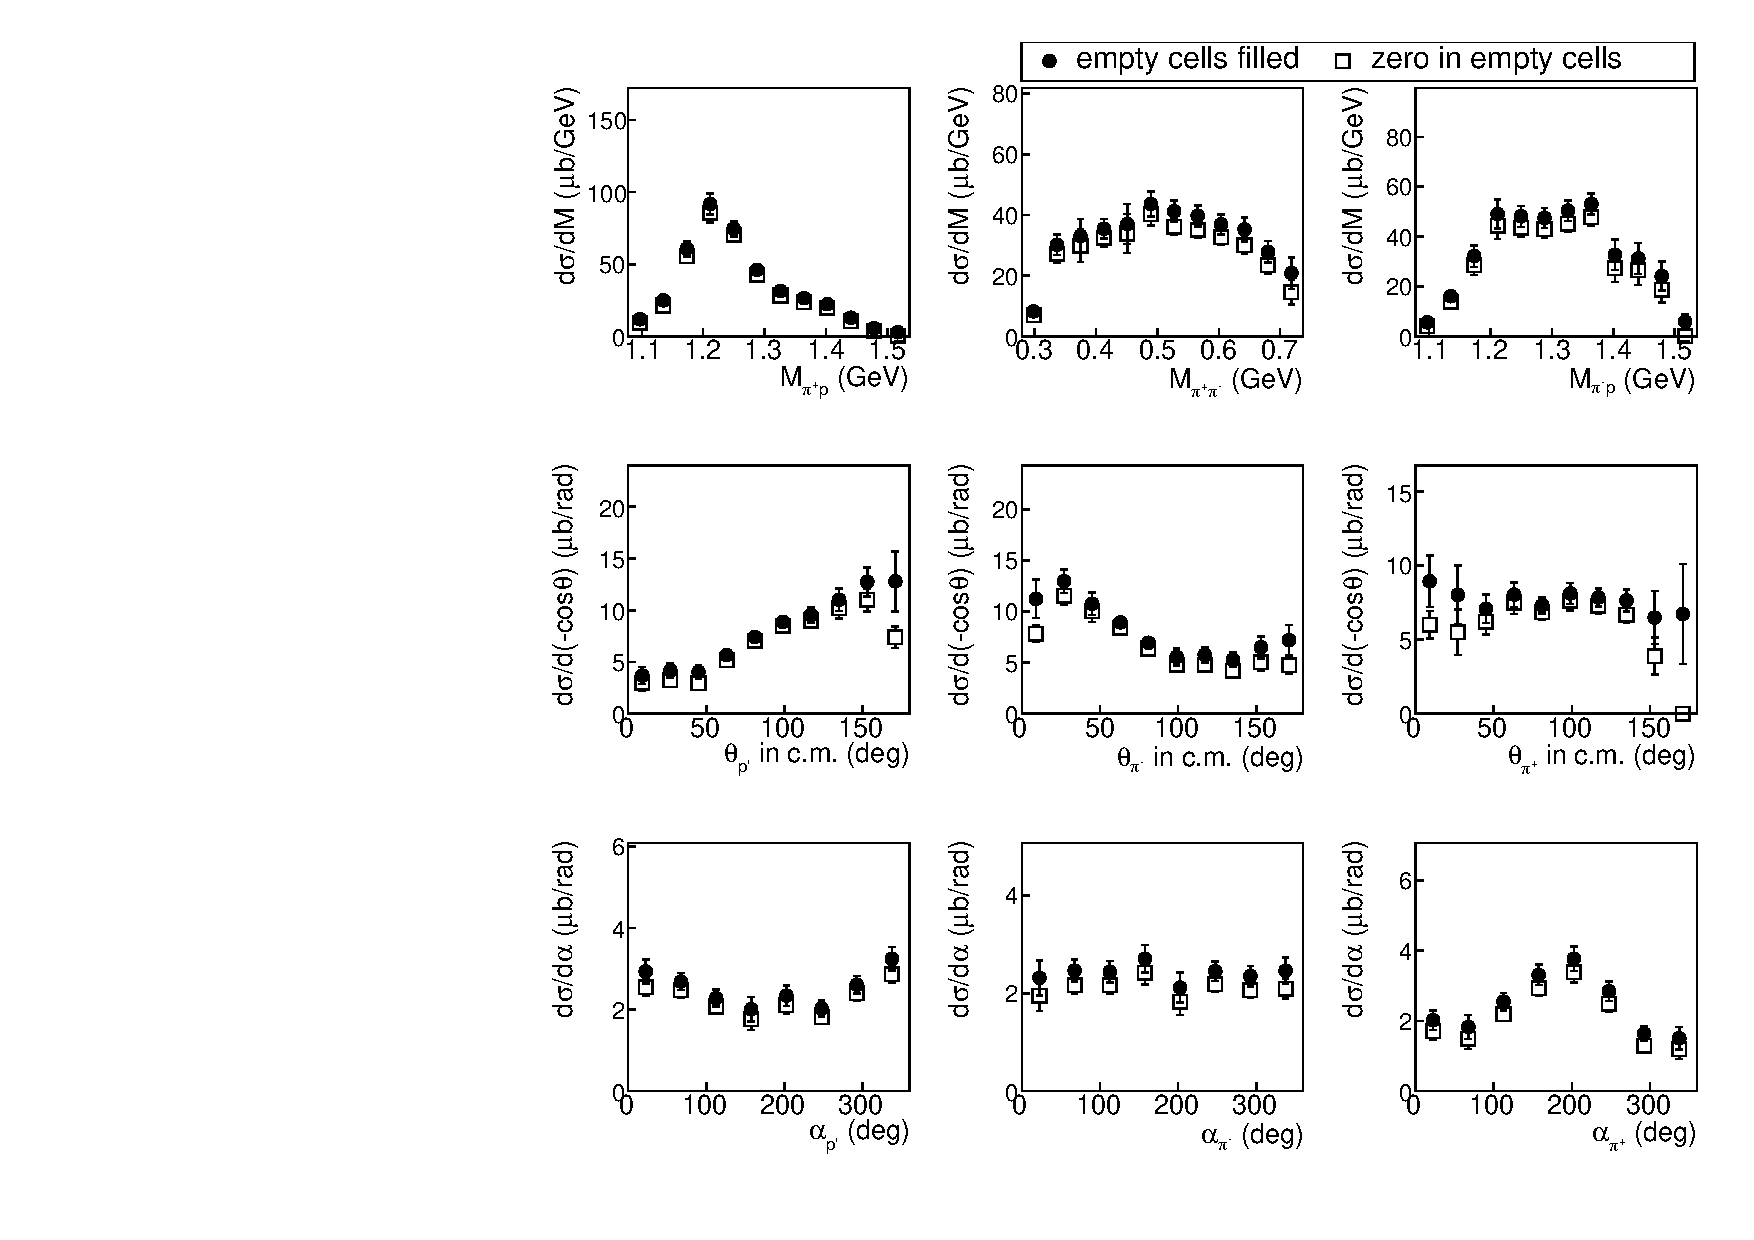
\includegraphics[width=13.75cm]{pictures/corrections/cr_sec_all_top_new.pdf}}
\caption{\small Extracted single-differential cross sections for the cases when the contribution from the empty cells was ignored (empty squares) and when it was taken into account (black circles). The former are reported with the uncertainty $\delta_{\text{stat}}^{\text{tot}}$ given by Eq.~\eqref{errortot}, while the latter are with the uncertainty $\delta_{\text{stat,mod}}^{\text{tot}}$ given by Eq.~\eqref{eq:error_stat_mod}. All distributions are given for one particular bin in $W$ and $Q^2$ ($W = $1.6375 GeV, $Q^2 = $0.625 GeV$^2$).} \label{fig:empt_corr}
\end{center}
\end{figure}


\begin{table}
\begin{center}
\caption{\small Relative empty cell contribution to the integral cross sections for all reported $(W,~Q^2)$-points. The columns correspond to the $Q^2$ values in GeV$^2$ and the rows to the $W$ values in GeV. Different shades of red correspond to different percentage range, i.e. the lightest shade corresponds to the contribution $\leq 20$\%, darker shade -- from 21\% to 30\%, and the darkest one shows the contribution $>30$\%.} \label{tab:int_empt_cont}
\resizebox{\textwidth}{!}{
\begin{tabular}{ ?c?c?c?c?c?c?c?c?c?c?c?c?c? } 
\Xhline{1.5pt}
        &           0.425       &         0.475        &         0.525         &           0.575       &          0.625       & 0.675                &        0.725         &         0.775        &          0.825       &         0.875        &         0.925        & 0.975\\ 
\Xhline{1.5pt}
 1.3125 & {\bf --}	        & \cellcolor{red!60}41 & \cellcolor{red!60}34  &  \cellcolor{red!60}32 & \cellcolor{red!60}35 & \cellcolor{red!60}37 & \cellcolor{red!60}41 & \cellcolor{red!60}33 & \cellcolor{red!60}33 & \cellcolor{red!60}45 & \cellcolor{red!60}35 & \cellcolor{red!60}48 \\ 
\Xhline{1.5pt}
 1.3375 & {\bf --}	        & \cellcolor{red!40}28 & \cellcolor{red!40}28  &  \cellcolor{red!40}27 & \cellcolor{red!40}26 & \cellcolor{red!40}28 & \cellcolor{red!60}31 & \cellcolor{red!60}32 & \cellcolor{red!60}33 & \cellcolor{red!60}35 & \cellcolor{red!60}33 & \cellcolor{red!60}35 \\ 
\Xhline{1.5pt}
 1.3625 & {\bf --} 	        & \cellcolor{red!40}28 & \cellcolor{red!40}26  &  \cellcolor{red!40}23 & \cellcolor{red!40}24 & \cellcolor{red!40}25 & \cellcolor{red!40}25 & \cellcolor{red!40}25 & \cellcolor{red!40}27 & \cellcolor{red!40}27 & \cellcolor{red!40}28 & \cellcolor{red!40}27 \\ 
\Xhline{1.5pt}
 1.3875 & {\bf --} 	        & \cellcolor{red!40}21 & \cellcolor{red!25}19  &  \cellcolor{red!25}18 & \cellcolor{red!25}17 & \cellcolor{red!25}19 & \cellcolor{red!25}19 & \cellcolor{red!25}18 & \cellcolor{red!25}18 & \cellcolor{red!40}21 & \cellcolor{red!40}23 & \cellcolor{red!40}21 \\ 
\Xhline{1.5pt}  
 1.4125 & {\bf --}	        & \cellcolor{red!40}27 & \cellcolor{red!25}20  &  \cellcolor{red!25}18 & \cellcolor{red!25}17 & \cellcolor{red!25}17 & \cellcolor{red!25}18 & \cellcolor{red!25}20 & \cellcolor{red!25}19 & \cellcolor{red!25}20 & \cellcolor{red!25}20 & \cellcolor{red!25}20 \\ 
\Xhline{1.5pt}
 1.4375 & {\bf --}	        & \cellcolor{red!40}23 & \cellcolor{red!25}17  &  \cellcolor{red!25}17 & \cellcolor{red!25}14 & \cellcolor{red!25}14 & \cellcolor{red!25}14 & \cellcolor{red!25}17 & \cellcolor{red!25}15 & \cellcolor{red!25}15 & \cellcolor{red!25}16 & \cellcolor{red!25}18 \\ 
\Xhline{1.5pt}
 1.4625 & {\bf --}	        & \cellcolor{red!40}21 & \cellcolor{red!25}16  &  \cellcolor{red!25}14 & \cellcolor{red!25}13 & \cellcolor{red!25}13 & \cellcolor{red!25}12 & \cellcolor{red!25}13 & \cellcolor{red!25}13 & \cellcolor{red!25}13 & \cellcolor{red!25}14 & \cellcolor{red!25}16 \\ 
\Xhline{1.5pt}
 1.4875 & {\bf --}	        & \cellcolor{red!40}24 & \cellcolor{red!25}18  &  \cellcolor{red!25}15 & \cellcolor{red!25}14 & \cellcolor{red!25}14 & \cellcolor{red!25}13 & \cellcolor{red!25}13 & \cellcolor{red!25}15 & \cellcolor{red!25}15 & \cellcolor{red!25}15 & \cellcolor{red!25}16 \\ 
 \Xhline{1.5pt}
 1.5125 & {\bf --}              & \cellcolor{red!40}23 & \cellcolor{red!25}18  &  \cellcolor{red!25}16 & \cellcolor{red!25}15 & \cellcolor{red!25}14 & \cellcolor{red!25}14 & \cellcolor{red!25}13 & \cellcolor{red!25}14 & \cellcolor{red!25}15 & \cellcolor{red!25}16 & \cellcolor{red!25}16\\ 
\Xhline{1.5pt}
 1.5375 & {\bf --}	        & \cellcolor{red!40}23 & \cellcolor{red!25}19  &  \cellcolor{red!25}16 & \cellcolor{red!25}16 & \cellcolor{red!25}14 & \cellcolor{red!25}14 & \cellcolor{red!25}14 & \cellcolor{red!25}14 & \cellcolor{red!25}17 & \cellcolor{red!25}18 & \cellcolor{red!25}15 \\ 
\Xhline{1.5pt}
 1.5625 & {\bf --}              & \cellcolor{red!40}22 & \cellcolor{red!25}19  &  \cellcolor{red!25}16 & \cellcolor{red!25}16 & \cellcolor{red!25}15 & \cellcolor{red!25}15 & \cellcolor{red!25}15 & \cellcolor{red!25}15 & \cellcolor{red!25}17 & \cellcolor{red!25}17 & \cellcolor{red!25}17 \\ 
\Xhline{1.5pt}
 1.5875 & {\bf --}              & \cellcolor{red!40}23 & \cellcolor{red!25}18  &  \cellcolor{red!25}17 & \cellcolor{red!25}20 & \cellcolor{red!25}15 & \cellcolor{red!25}15 & \cellcolor{red!25}17 & \cellcolor{red!25}16 & \cellcolor{red!25}18 & \cellcolor{red!25}17 & {\bf --}\\ 
\Xhline{1.5pt}
 1.6125 & \cellcolor{red!40}26  & \cellcolor{red!25}20 & \cellcolor{red!25}17  &  \cellcolor{red!25}16 & \cellcolor{red!25}15 & \cellcolor{red!25}15 & \cellcolor{red!25}15 & \cellcolor{red!25}15 & \cellcolor{red!25}17 & \cellcolor{red!25}16 & \cellcolor{red!25}15 & {\bf --}\\ 
 \Xhline{1.5pt}
 1.6375 & \cellcolor{red!40}26  & \cellcolor{red!25}19 & \cellcolor{red!25}17  &  \cellcolor{red!25}16 & \cellcolor{red!25}14 & \cellcolor{red!25}16 & \cellcolor{red!25}14 & \cellcolor{red!25}16 & \cellcolor{red!25}17 & \cellcolor{red!25}16 & {\bf --}             & {\bf --} \\
\Xhline{1.5pt}
 1.6625 & \cellcolor{red!40}25  & \cellcolor{red!25}19 & \cellcolor{red!25}17  &  \cellcolor{red!25}15 & \cellcolor{red!25}15 & \cellcolor{red!25}15 & \cellcolor{red!25}15 & \cellcolor{red!25}17 & \cellcolor{red!25}18 & \cellcolor{red!25}17 & {\bf --}             & {\bf --} \\ 
\Xhline{1.5pt}
 1.6875 & \cellcolor{red!40}24  & \cellcolor{red!25}20 & \cellcolor{red!25}17  &  \cellcolor{red!25}16 & \cellcolor{red!25}15 & \cellcolor{red!25}15 & \cellcolor{red!25}16 & \cellcolor{red!25}19 & \cellcolor{red!25}18 & {\bf --}             & {\bf --}             & {\bf --} \\ 
\Xhline{1.5pt}
 1.7125 & \cellcolor{red!40}23  & \cellcolor{red!25}19 & \cellcolor{red!25}17  &  \cellcolor{red!25}17 & \cellcolor{red!25}16 & \cellcolor{red!25}17 & \cellcolor{red!25}19 & \cellcolor{red!25}18 & {\bf --}             & {\bf --}             & {\bf --}             & {\bf --} \\ 
 \Xhline{1.5pt}
 1.7375 & \cellcolor{red!40}23  & \cellcolor{red!25}20 & \cellcolor{red!25}17  &  \cellcolor{red!25}17 & \cellcolor{red!25}17 & \cellcolor{red!25}18 & \cellcolor{red!25}19 & {\bf --}             & {\bf --}             & {\bf --}             & {\bf --}             & {\bf --} \\
\Xhline{1.5pt}
 1.7625 & \cellcolor{red!40}22  & \cellcolor{red!25}20 & \cellcolor{red!25}18  &  \cellcolor{red!25}18 & \cellcolor{red!25}18 & \cellcolor{red!25}19 & {\bf --}             & {\bf --}             & {\bf --}             & {\bf --}             & {\bf --}             & {\bf --} \\ 
\Xhline{1.5pt}
 1.7875 & \cellcolor{red!40}21  & \cellcolor{red!25}19 & \cellcolor{red!25}18  &  \cellcolor{red!25}18 & {\bf --}             & {\bf --}             & {\bf --}             & {\bf --}             & {\bf --}             & {\bf --}             & {\bf --}             & {\bf --} \\
\Xhline{1.5pt}
 1.8125 & \cellcolor{red!40}21  & \cellcolor{red!25}17 &{\bf --}               &{\bf --}               & {\bf --}             & {\bf --}             & {\bf --}             & {\bf --}             & {\bf --}             & {\bf --}             & {\bf --}             & {\bf --} \\ 
\Xhline{1.5pt}
\end{tabular}}
\end{center}
\end{table}


%\begin{enumerate}

%\item The map of the empty cells is determined using the Monte Carlo simulation. For that purpose, firstly, so-called unit generated histogram and unit reconstructed histogram are obtained as\footnote[4]{All operation with the multi-dimensional histograms given here are implied to be performed with the contents of the corresponding multi-dimensional bins.}

%\begin{equation}
%\begin{aligned}
%&h\_5d\_unit\_gen&=~& h\_5d\_gen/h\_5d\_gen,\\
%&h\_5d\_unit\_rec&=~& h\_5d\_rec/h\_5d\_rec.
%\end{aligned}
%\end{equation}
%These unit histograms have 1 in that bins that were filled and 0 in empty bins.

%Then, the map of the empty cells is obtained as 

%\begin{equation}
%\begin{aligned}
%h\_5d\_map &= h\_5d\_unit\_gen - h\_5d\_unit\_rec.
%\end{aligned}
%\end{equation}

%This unit histogram has 1 in bins where we have generated, but do not have reconstructed, and 0 in other bins.

%\item 

%\end{enumerate}

%F_{data}^{int} = \int [h\_5d\_data/h\_5d\_unit\_rec]\\
%F_{gen}^{int} = \int [h\_5d\_gen/h\_5d\_unit\_rec]\\
%F_{eff}^{avrg} = \frac{1}{N_{bins}} \int [h\_5d\_eff]\\

%\newpage


\section{Radiative correction}
\label{Sect:rad_corr}

The incoming and scattered electrons are subject to radiative effects, which means that they can emit photons thus reducing their energy. However, in the experiment the information on these emissions is not accessible, and one has to assume the electron energy to be unchanged. Therefore, when extracting the cross sections, one assumes the energy of the incoming/scattered electron to be greater/smaller than it actually was in the reaction. This, in turn, leads to the systematic overestimation of the virtual photon energy with the consequent overestimation\footnote[2]{The $Q^2$ value is overestimated if the incoming electron emits and underestimated if the scattered electron emits. That is why the radiative effects do not significantly impact the $Q^{2}$-dependence of the cross section.} of $W$. As a result, the extracted cross section is assigned to the $W$ value higher than the actual one. This distorts the measured $W$ spectrum and leads to its agglomeration in the high-lying region.


The common way of handling this problem is to apply the radiative correction to the extracted cross sections. In this study the radiative correction is performed using TWOPEG-D~\cite{twopeg-d}, which is the event generator for the double-pion electroproduction that simulates effects of the target motion. TWOPEG-D accounts for the radiative effects by means of the well-known approach of Ref.~\cite{Mo:1968cg}, which is traditionally used for the radiative corrections in the studies of double-pion electroproduction~\cite{Rip_an_note:2002,Ripani:2002ss,Fed_an_note:2007,Fedotov:2008aa,Fed_an_note:2017,Fed_paper_2018,Isupov:2017lnd,Arjun}. In Ref.~\cite{Mo:1968cg} the approach is applied to the inclusive case, while in TWOPEG-D, the double-pion integrated cross sections are used instead~\cite{twopeg,twopeg-d}. 

In the approach~\cite{Mo:1968cg,twopeg,twopeg-d} the radiative photons are supposed to be emitted collinearly either to the direction of the incoming or scattered electron (the so-called ``peaking approximation"). The calculation of the radiative cross section is split into two parts. The ``soft" part assumes the energy of the emitted radiative photon to be less than a certain minimal value (10 MeV), while the ``hard" part is for the photons with an energy greater than that value. The ``soft" part is evaluated explicitly, while for the calculation of the ``hard" part, an inclusive hadronic tensor is assumed. The latter assumption is however considered adequate, especially taking into account that approaches that are capable of describing radiative processes in exclusive double-pion electroproduction are not yet available.


The radiative correction factor $R$ in Eq.~\eqref{expcrossect} is determined in the following way. The double-pion events either with or without radiative effects are generated with TWOPEG-D. Both radiated and non-radiated events are subjected to the smearing due to the Fermi motion of the target. Then the ratio given by Eq.~\eqref{eq:rad_corr} is taken in each $\Delta W \Delta Q^{2}$ bin.
\begin{equation}
R(\Delta W, \Delta Q^{2}) = \frac{\mathbb{N}_{rad}}{\mathbb{N}_{norad}},
\label{eq:rad_corr}
\end{equation}
where $\mathbb{N}_{rad}$ and $\mathbb{N}_{norad}$ are the weighted numbers of generated events in each $\Delta W \Delta Q^{2}$ bin with and without radiative effects, respectively. Note that neither $\mathbb{N}_{rad}$ nor $\mathbb{N}_{norad}$ are subject to any cuts.

\begin{figure}[htp]
\begin{center}
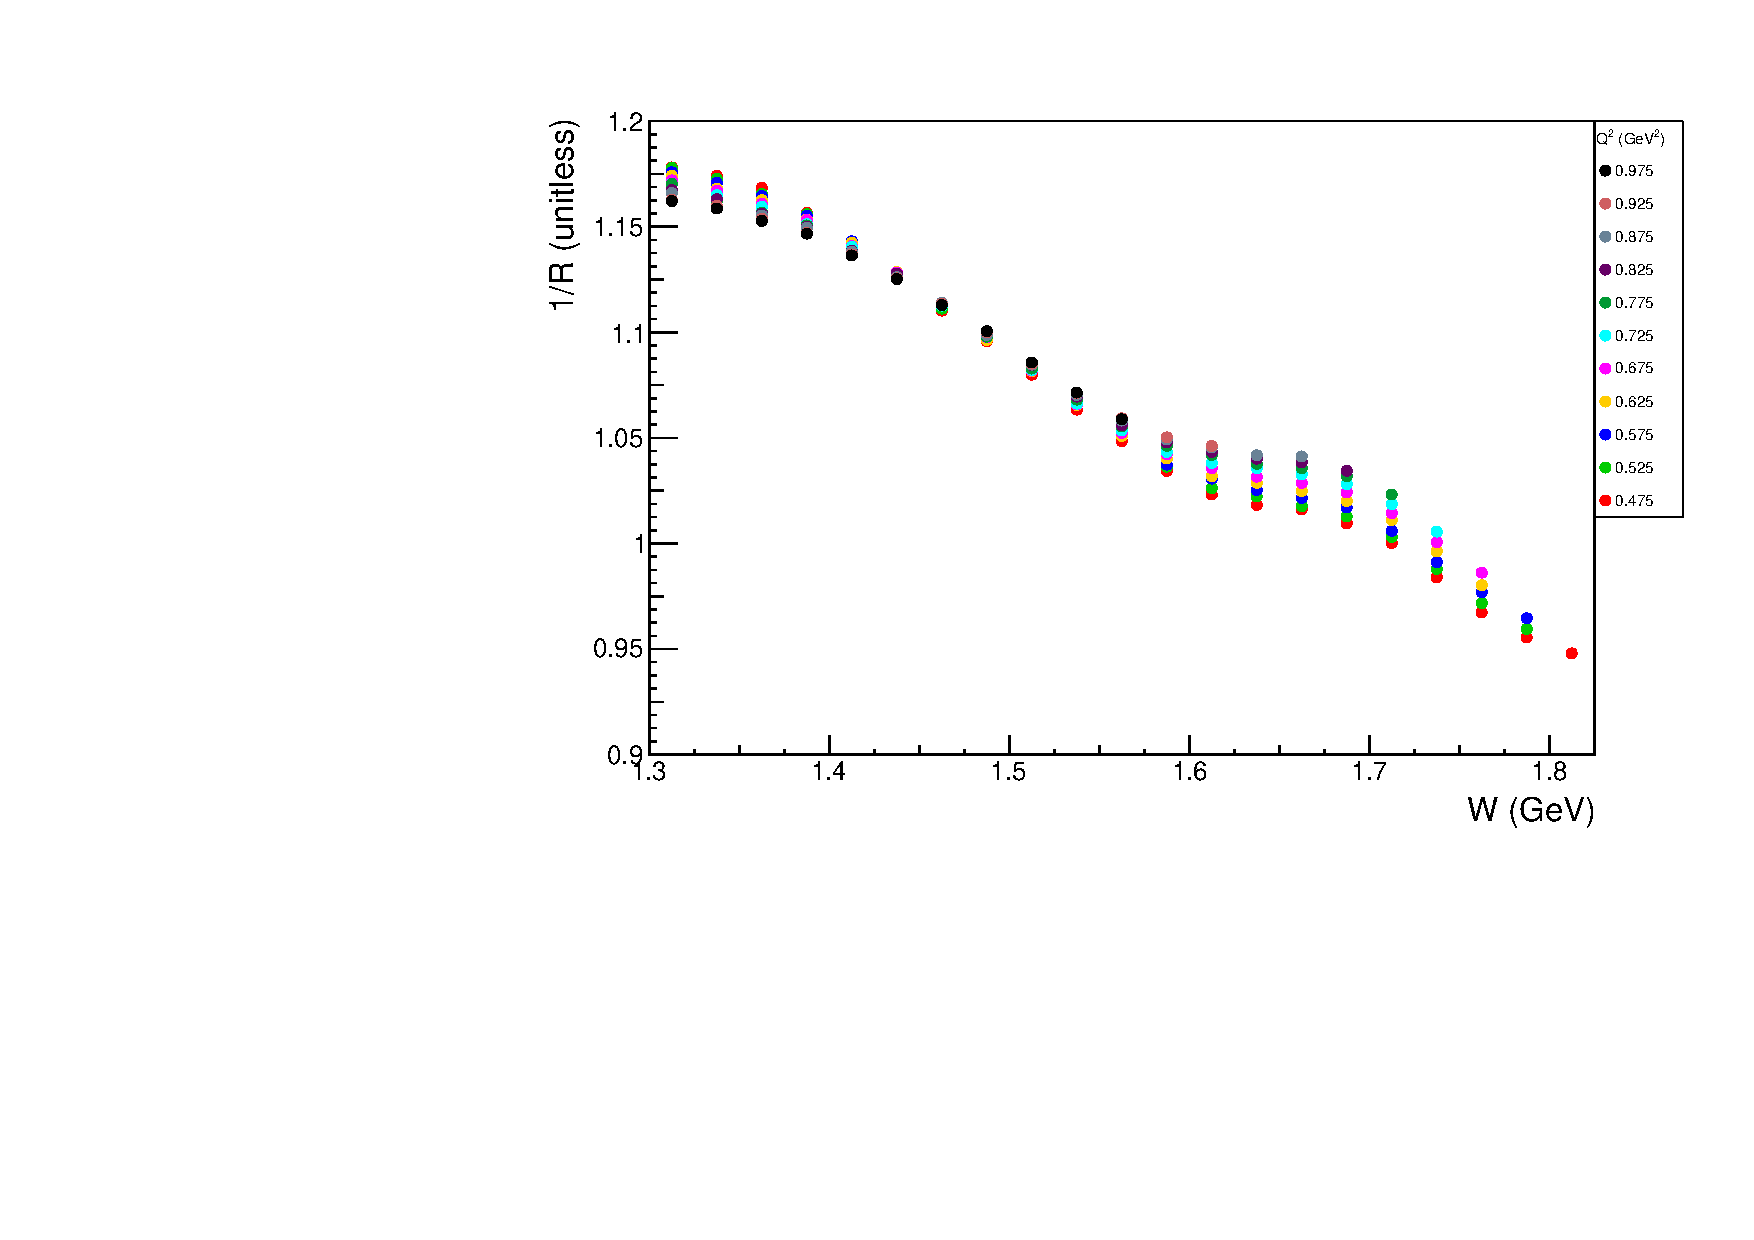
\includegraphics[width=13cm]{pictures/corrections/radcorr.pdf}
\caption{\small Reciprocal of the radiative correction factor ($1/R$) as a function of $W$ for different $Q^{2}$ bins (see Eq.~\eqref{eq:rad_corr}).} \label{fig:radcorr}
\end{center}
\end{figure}

This approach gives the correction factor $R$ only as a function of $W$ and $Q^{2}$, disregarding its dependence on the hadronic variables. However, the need to integrate the cross section at least over four hadronic variables (see Eq.~\eqref{inegr5diff}) considerably reduces the influence of the final state hadron kinematics on the radiative correction factor, thus justifying the applicability of the procedure~\cite{Mo:1968cg,twopeg,twopeg-d}.

The quantity $1/R$ is plotted in Fig.~\ref{fig:radcorr} as a function of $W$ for different $Q^{2}$ bins. The uncertainties associated with the statistics of generated events are very small and therefore not seen in the plot\footnote[3]{The total of about 2.5$\cdot 10^{9}$ either radiated or non-radiated events were generated in the investigated kinematic region for the calculation of the radiative correction factor.}. Note that the correction factor introduced in Fig.~\ref{fig:radcorr} is slightly different from that given in Ref.~\cite{Fed_an_note:2017} for the same beam energy of the free proton experiment ($E_{beam} = 2.039$~GeV). This difference comes from the fact that generated events in Eq.~\eqref{eq:rad_corr} are subjected to the smearing due to the Fermi motion of the target proton. 

Once this correction is applied, the extracted cross sections are treated as non-radiated, but Fermi-smeared.


\section{Unfolding the effects of the target motion}
\label{Sect:fermi_corr}


The motion of the target proton in a deuterium nucleus introduces into this analysis some specific issues that are not inherent for the previously conducted studies of the double-pion cross sections~\cite{Rip_an_note:2002,Ripani:2002ss,Fed_an_note:2007,Fedotov:2008aa,Isupov:2017lnd,Arjun,Fed_an_note:2017,Fed_paper_2018}. As was described in Sects.~\ref{Sect:excl_cut} and~\ref{Sect:smearing_blurring}, the intention to use in the analysis the $\pi^{-}$ missing topology (that serves the purpose of the cross section extraction best) leads inevitably to working under the target-at-rest-assumption. The latter, however, not only complicates the selection of exclusive events (see Sect.~\ref{Sect:excl_cut}), but also impacts the extracted cross sections due to the following reasons.

\begin{itemize}

\item  One has to use the smeared reaction invariant mass $W_{sm}$ for the cross section binning (see Sect.~\ref{Sect:smearing_blurring}). As a result, the extracted cross section is assigned to the $W$ value different from the actual one. This makes both integral and single-differential cross sections to be distorted. 

 
\item  One has to use an approximate Lab to CMS transformation that ignores the target motion (see Sect.~\ref{Sect:lab_cms}). This approximation introduces some inaccuracy to the measured angular ($\theta$, $\varphi$, and $\alpha$) distributions without having an impact on the invariant mass distributions and $W$ and $Q^{2}$ cross section dependencies due to their Lorentz invariance. 


\end{itemize}

The former effect is thought to have a much greater impact on the cross section than the latter. Thus, being folded with the aforementioned effects of the target motion, the extracted cross sections are seeking the corresponding unfolding correction. This correction is performed by means of two Monte Carlo event generators TWOPEG~\cite{twopeg} and TWOPEG-D~\cite{twopeg-d}. TWOPEG is the event generator for the double-pion electroproduction off the free proton that currently provides the best cross section estimation in the investigated kinematic region. TWOPEG-D is the event generator for the same exclusive reaction but off the proton that moves in the deuterium nucleus. This event generator was especially developed to be used in the studies, where the experimental information of the target proton momentum is inaccessible, and one is forced to work under the target-at-rest-assumption. TWOPEG-D convolutes the double-pion cross section with effects of the target motion and thus imitates the conditions of the experimental cross section extraction.

To calculate the correction factor, two samples of double-pion events produced either off the proton at rest and off the moving proton were generated (with TWOPEG and TWOPEG-D, respectively). Both event generators provide the particle's four-momenta written in the Lab system and distribute events according to the corresponding electron-scattering cross section. As the reaction invariant mass both samples use the value calculated from the initial particles (see Eq.~\eqref{W_fin_1}), which for the ``moving proton" events is calculated under the target-at-rest-assumption (as was done for the cross section calculation). The generated four-momenta are then subject to the transformation to the CMS. For both samples the transformation is performed according to the procedure given in App.~\ref{app_lab_cms_trans} for the case of the proton at rest. For the ``moving proton" sample, this approximation introduces in the event distributions the same inaccuracy as appears in the extracted cross sections. Then the kinematic variables are calculated and the generated events of both samples are binned in the same way as the extracted cross sections (see Sect.~\ref{Sect:binning}). 


\begin{figure}[htp]
\begin{center}
\framebox{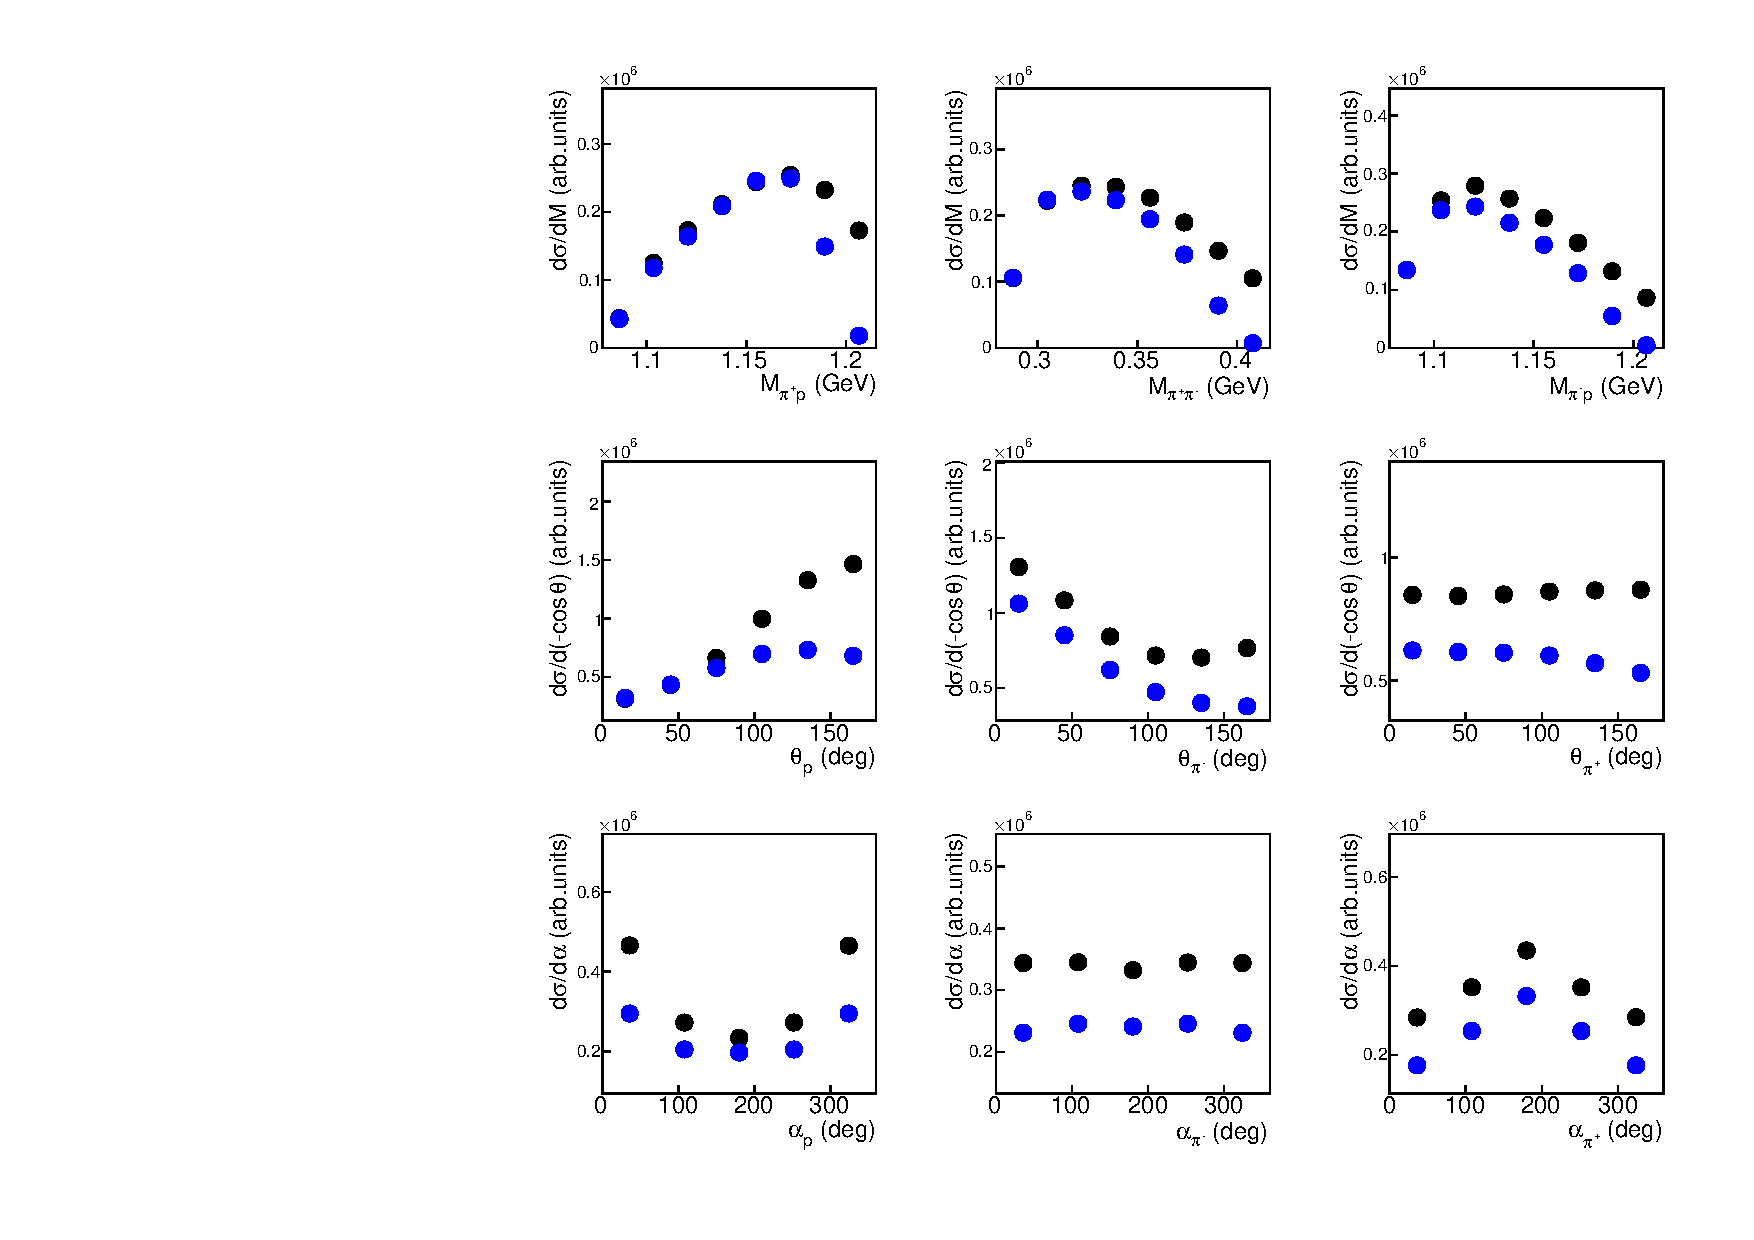
\includegraphics[width=12cm]{pictures/corrections/ferm_noferm_1diff_475_13375.pdf}}
\caption{\small Single-differential distributions of generated double-pion events produced off the proton at rest (blue symbols) and off the moving proton (black symbols). The former were generated with TWOPEG~\cite{twopeg} and the latter with TWOPEG-D~\cite{twopeg-d}. The example is given for the particular $\Delta W \Delta Q^{2}$ bin with the central point at $W=1.3375$~GeV and $Q^{2}=0.475$~GeV$^{2}$. As this bin is located near the threshold, the moving proton distributions (black symbols) have a high relative event excess comparing with the free proton distributions (blue symbols). See text for details. } \label{ferm_cor_1diff_1}
\end{center}
\end{figure}

Therefore, the distributions of events generated with TWOPEG-D acquire the same inaccuracies as the extracted cross sections, i.e. the value $W_{sm}$ is used for the binning and the approximate Lab to CMS transformations are applied. The manifestation of these inaccuracies differs depending on various final state variables and has a strong $W$-dependence as Figs.~\ref{ferm_cor_1diff_1} and~\ref{ferm_cor_1diff_2} demonstrate. These figures show the single-differential distributions of $\mathbb{N}_{nofermi}$ (blue symbols) and $\mathbb{N}_{fermi}$ (black symbols), which are the weighted numbers of events generated with TWOPEG and TWOPEG-D, respectively. In Fig.~\ref{ferm_cor_1diff_1} these distributions are shown for a low $W = 1.3375$~GeV, while in Fig.~\ref{ferm_cor_1diff_2} they are shown for a higher $W=1.5625$~GeV. The uncertainties associated with the statistics of generated events are very small and therefore not seen in the plots\footnote[4]{For each event sample the total of about 2.5$\cdot 10^{10}$ events were generated in the investigated kinematic region for the calculation of the correction factor.}.

\begin{figure}[htp]
\begin{center}
\framebox{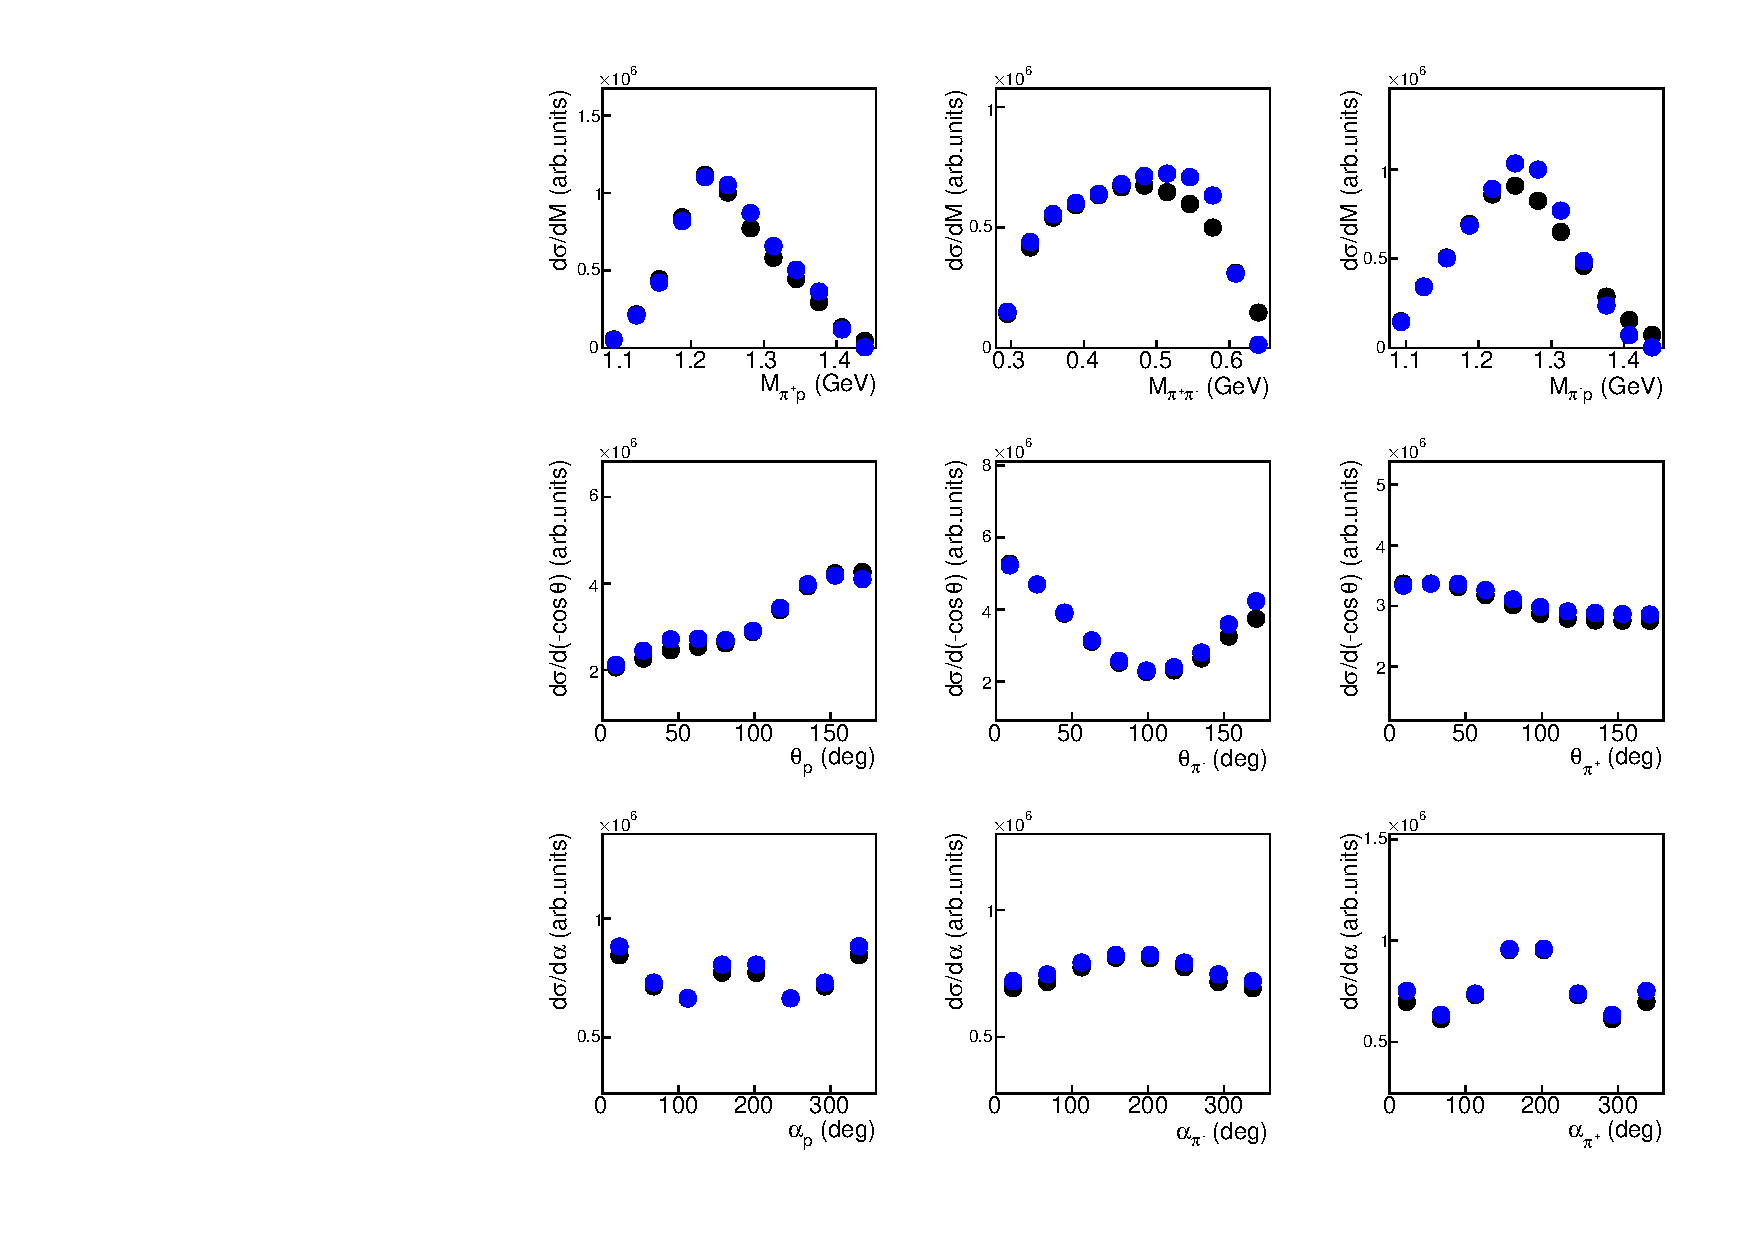
\includegraphics[width=12cm]{pictures/corrections/ferm_noferm_1diff_475_15625.pdf}}
\caption{\small Single-differential distributions of generated double-pion events produced off the proton at rest (blue symbols) and off the moving proton (black symbols). The former were generated with TWOPEG~\cite{twopeg} and the latter with TWOPEG-D~\cite{twopeg-d}. The example is given for the particular $\Delta W \Delta Q^{2}$ bin with the central point at $W=1.5625$~GeV and $Q^{2}=0.475$~GeV$^{2}$. As the bin is located in the peak region, the moving proton distributions (black symbols) have a small relative event deficit comparing with the free proton distributions (blue symbols). See text for details. } \label{ferm_cor_1diff_2}
\end{center}
\end{figure}

As seen from Figs.~\ref{ferm_cor_1diff_1} and~\ref{ferm_cor_1diff_2}, the target motion considered under the itemized conditions listed above affects mostly the cross section near the threshold, while for higher $W$ their impact is significantly less pronounced. This happens due to the following. Let's consider a particular $W_{true}$ bin. As shown in Ref.~\cite{twopeg-d}, each value of $W_{true}$ corresponds to a sequence of $W_{sm}$ values, which are symmetrically scattered in the vicinity of $W_{true}$ with a spread of 50-100 MeV. This leads to the fact that the same bin in $W_{sm}$ has a different number of events compared to the $W_{true}$ bin. This difference depends on the cross section behavior in the vicinity of 50-100 MeV of this bin. The cross section abruptly rises from the threshold with a strong convex nonlinearity, which smooths as $W$ grows up to 1.4~GeV, and then turns to a concave nonlinearity forming the left slope of the resonance peak at 1.5~GeV. Then the cross section modestly increases and decreases several times changing its nonlinearity type. In any $W_{true}$ subrange the cross section can be written as $a + f(W)$, where $a=const$, while $f(W)$ evolves from zero and determines the cross section nonlinearity within the subrange.  Then the absolute variation in the event number in $W_{sm}$ bin is determined solely by the nonlinearity of the function $f(W)$, i.e. convex nonlinearity leads to an event excess in the bin, while concave nonlinearity -- to an event deficit. Hence, in the resonance peaks an event deficit is observed, while the region close to the threshold and the dip between the peaks have an event excess. However, the relative event variation depends on $a$ and is higher for smaller $a$. The smallest value of $a$ is reached at the threshold ($a = 0$), therefore the near-to-threshold subrange has the greatest relative variation of event number.



Indeed, in Fig.~\ref{ferm_cor_1diff_1}, which is plotted for the $W$ bin located close to the threshold, the moving proton distributions (black symbols) have a high relative event excess compared to the free proton distributions (blue symbols). Meanwhile, in Fig.~\ref{ferm_cor_1diff_2}, which is plotted for the $W$ bin located at the peak region, the moving proton distributions (black symbols) have small relative event deficit comparing with the free proton distributions (blue symbols). 

For the low $W$ region (as in Fig.~\ref{ferm_cor_1diff_1}) it is noteworthy that a very large relative difference between the free proton and the moving proton cross sections is observed for the right part of the invariant mass distributions. This happens due to the phase space broadening with $W$ that takes place for invariant masses (see App.~\ref{app_ph_space}). The invariant mass distribution typically has a maximum in the middle and gradually goes to zero on both edges. The lower the $W$ value is, the narrower is the distribution width. As $W$ grows, the distribution widens to the right and goes to zero farther away. Meanwhile, each bin in $W_{sm}$ contains a mixture of events with the values of $W_{true}$ spread within 50-100~MeV near this bin. For low $W$ this spread is comparable with the total  width of the invariant mass distribution. Therefore, the right distribution side acquired the event excess that comes from the same bins in invariant mass but located at higher $W_{true}$ and hence having high cross sections.


The unfolding correction is performed in each multi-dimensional bin of the double-pion production phase-space (see Sect.~\ref{Sect:kin_var} as well as App.~\ref{app_ph_space}), i.e. in each $\Delta W \Delta Q^{2}\Delta^{5}\tau$ bin the cross section is divided by the correction factor $\mathcal{F}$ (see  Eq.~\eqref{expcrossect}) that is calculated as
\begin{equation}
\mathcal{F}(\Delta W, \Delta Q^{2},\Delta^{5}\tau) = \frac{\mathbb{N}_{fermi}}{\mathbb{N}_{nofermi}},
\label{eq:ferm_corr}
\end{equation}
where $\mathbb{N}_{nofermi}$ and $\mathbb{N}_{fermi}$ are the weighted numbers of generated double-pion events in the $\Delta W \Delta Q^{2}\Delta^{5}\tau$ bin produced off the proton at rest and off the moving proton, respectively. Both event samples were generated without radiative effects, since the correction factor $\mathcal{F}$ is applied to the cross sections that are already corrected for the radiative effects (see Sect.~\ref{Sect:rad_corr}).


The impact of the unfolding correction on the extracted integral cross sections is illustrated in Fig.~\ref{ferm_cor_nocor_int}, where the distributions before the correction are plotted in orange, while the distributions after the correction are plotted in dark blue. The comparison is given for two $Q^{2}$ bins. As was expected, the correction causes a slight cross section increase in the resonance peaks and a decrease near the threshold and in the dip between the peaks. 

\begin{figure}[htp]
\begin{center}
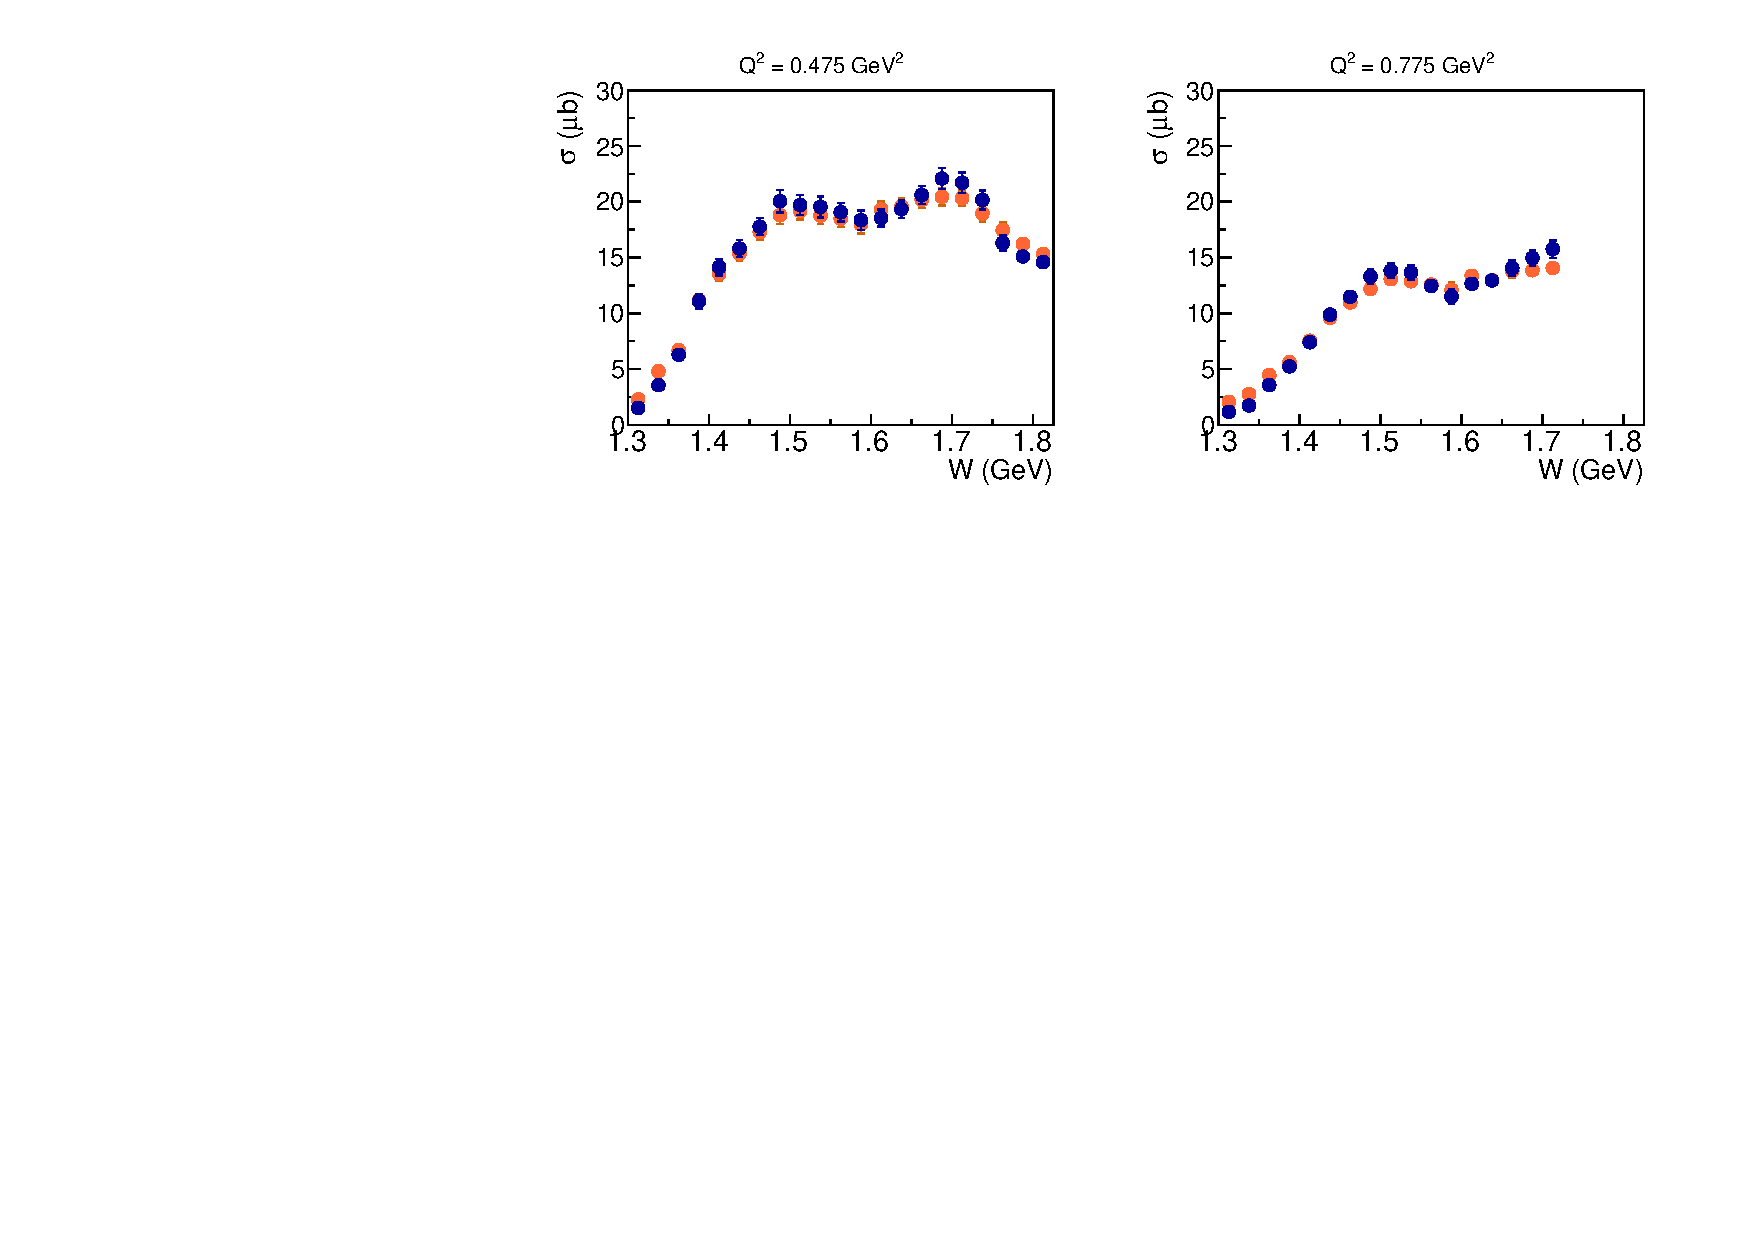
\includegraphics[width=14cm]{pictures/corrections/fermi_cor_nocor_int.pdf}
\caption{\small Impact of the unfolding correction on the extracted integral cross sections. The cross section before the correction is plotted in orange, while the cross section after the correction is plotted in dark blue (both are divided by the virtual photon flux). The comparison is given for two $Q^{2}$ bins as specified above the plots. } \label{ferm_cor_nocor_int}
\end{center}
\end{figure}

The value of the correction factor in Eq.~\eqref{eq:ferm_corr} depends on both the free proton cross sections and the model of the deuteron wave function that were employed in the event generators. The former relies strongly on the JM model fit of the available data on double-pion cross sections, while for the latter the Bonn model was used (see Refs.~\cite{twopeg,twopeg-d} for more detail). Therefore, the uncertainty of the extracted cross sections that comes from this unfolding correction is attributed to the model dependence uncertainty and is discussed in Sect.~\ref{Sect:mod_dep}. 

Once corrected for the effects of the target motion and then divided by the virtual photon flux, the cross section is treated as the true virtual photoproduction cross section and is attributed to the central point of the corresponding $\Delta W \Delta Q^{2}\Delta^{5}\tau$ bin.


\section{Correction for binning effects}
\label{Sect:bin_cor}

The cross section, extracted in bins of a finite size, is assigned to the central point of a bin. On this way the cross sections acquire binning caused distortions and, therefore, are seeking the corresponding corrections. In this section, which is devoted to the binning effects, two separate binning issues are distinguished, i.e. (i) the specific issue of affecting the cross section value in the next to last point of the invariant mass distributions and (ii) the common binning issue that impacts the cross section value in any bin of finite size. 

Let's address the specific binning issue in the invariant mass distributions first. As shown in Sect.~\ref{Sect:binning}, the binning in invariant mass requires special attention due to the broadening of the reaction phase-space with $W$ (see App.~\ref{app_ph_space}) and the corresponding $W$ dependence of the upper boundary of the invariant mass distributions (see Eq.~\eqref{eq:inv_mass_boundary}). This effect makes the upper boundary $M_{upper}$ to be indistinct, since the cross section is calculated in a bin $W_{left} < W < W_{right}$. To deal with this difficulty, the value of $M_{upper}$ is calculated using $W_{center}$, the center of the $W$ bin. Then a specific arrangement of mass bins is used, which forces the last bin to be situated completely out of the boundaries given by Eq.~\eqref{eq:inv_mass_boundary} using $W_{center}$. When integrating the cross section over the mass distribution, the events in the extra bin are included, but a cross section for this bin is not reported.


Meanwhile, the cross section in the next to last bin (labeled as bin number $N_{bins}-1$) should be treated carefully. This is best illustrated in Fig.~\ref{fig:mass_corr}, which shows schematically the event distribution in mass, ending in $M_{upper}$ for three choices of $W$ at $W_{left}$ (dot-dashed), $W_{center}$ (solid) and $W_{right}$ (dashed). The black points at $M^{N_{bins}-1}_{left}$ and $M^{N_{bins}-1}_{right}$ show the left and right boundaries of the next to last bin, respectively. In the next to last bin events with $W < W_{center}$ are distributed over a range, which is less than $\Delta M$ defined by Eq.~\eqref{eq:bin_width}. However, when extracting the cross sections, the event yield was divided by the full bin width $\Delta M$, thus leading to an underestimation of the cross section.



\begin{figure}[htp]
\begin{center}
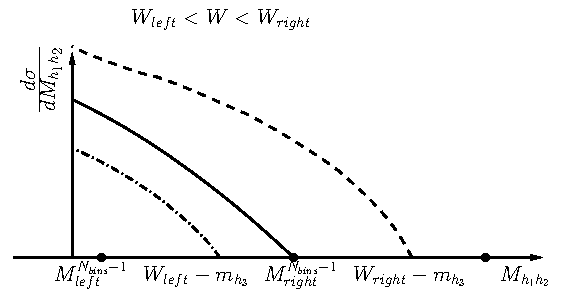
\includegraphics[width=12cm]{pictures/corrections/mass_tex.pdf}
\caption{\small  Schematic representation of the invariant mass distributions ending in $M_{upper}$ calculated according to Eq.~\eqref{eq:inv_mass_boundary} for three choices of $W$ at $W_{left}$ (dot-dashed), $W_{center}$ (solid) and $W_{right}$ (dashed). The black points at $M^{N_{bins}-1}_{left}$ and $M^{N_{bins}-1}_{right}$ show the left and right boundaries of the next to last bin, respectively, while the remaining point marks the right boundary of the last mass bin.} \label{fig:mass_corr}
\end{center}
\end{figure}


The correction for this effect was taken from Ref.~\cite{Fed_an_note:2017,Fed_paper_2018}. It was made using the TWOPEG double-pion event generator~\cite{twopeg}. The correction factor to the cross section in the next to last bin is the ratio of the simulated cross sections calculated with fixed $\Delta M$ defined by Eq.~\eqref{eq:bin_width} and with $\widetilde{\Delta M} = W-m_{h_{3}} - M^{N_{bins}-1}_{left}$, which was different for each generated event. This factor provides the correction to the cross section in the next to last bin that varied from $\sim$5\% to $\sim$10\%.


Let's now address the common binning issue that impacts the cross section value in any bin of a finite size. Extracted in a finite bin, the cross section is subject to averaging within this bin. For instance, if there is a sharp peak in the middle of a bin, then the average value of the cross section in that bin will always be smaller than the peak value. Any non-linear behavior of the cross section will likely result in an offset of the obtained value. There are two methods of correcting this offset, i.e. (i) to correct the kinematic quantities associated with the bin and use the corrected values instead of the central values or (ii) to correct the cross section value in the center of the bin. Both these methods are widely used for the binning corrections. In the studies of double-pion cross sections, however, the second method has become conventional~\cite{Fed_an_note:2007,Fedotov:2008aa,Fed_an_note:2017,Fed_paper_2018}. Therefore, in this study the second method is chosen, in order to keep the initial binning over the kinematic variables and to facilitate the cross section comparison with the results obtained off the proton at rest~\cite{Fed_an_note:2017,Fed_paper_2018}.

In this study one-dimensional binning corrections are performed, i.e., the cross section dependence on each kinematic variable $x$ is corrected individually (where $x$ corresponds to $W$, $Q^{2}$, and hadron variables). In any one-dimensional bin $[x_{min},x_{max}]$ the cross section value is multiplied by the correction factor $C_{bin}$. To estimate this factor some assumptions about the cross section behavior within the bin are needed, and hence, the cross section shape should be described by a continuous function $f(x)$. The multiplicative correction factor $C_{bin}$ is then calculated in each bin $[x_{min},x_{max}]$ as
\begin{equation}
\begin{aligned}
%\sigma_{corr} & = &\sigma_{uncorr} \times
%C_{bin} & \text{ \,\,with}\\
\label{eq:bincor}
C_{bin} & = &\frac{f(x_{center})}{\int\limits_{x_{min}}^{x_{max}} f(x)dx} \textrm{ ,}
\end{aligned}  
\end{equation}
where $x_{center}$ is the central point of the $[x_{min},x_{max}]$ bin.






For the single-differential distributions a cubic spline approximation is chosen to continuously describe the cross section shape, as shown in Fig.~\ref{fig:bin_cor_1d}. The black and red points in this figure are the cross sections before and after binning corrections, respectively, and the curves correspond to the spline approximation. For the invariant mass and $\theta$ angular distributions the splines are forced to pass through the intermediate points that are obtained by averaging over two neighboring cross section points. This method reduces the splines sensitivity to accidental cross section fluctuations. Beside this, for the invariant mass distributions the splines are required to give zero at the distribution edges. For the $\alpha$ angular distributions the splines are forced to pass through the points that are obtained by averaging over two cross section points symmetrical with respect to $\alpha = 180^{\rm o}$. This approach reflects the fact that after the integration over $\varphi$, the cross section must be symmetrical in the $\alpha$ angle (meanwhile, the extracted experimental distributions are slightly asymmetrical)\footnote[5]{Although the $\varphi$ distributions are not reported here, they were nevertheless extracted and added to the CLAS physics database~\cite{CLAS_DB}. The $\varphi$ distributions were thus subjected to the binning correction with the same approach used for the $\theta$ distributions.}.

\begin{figure}[htp]
\begin{center}
\framebox{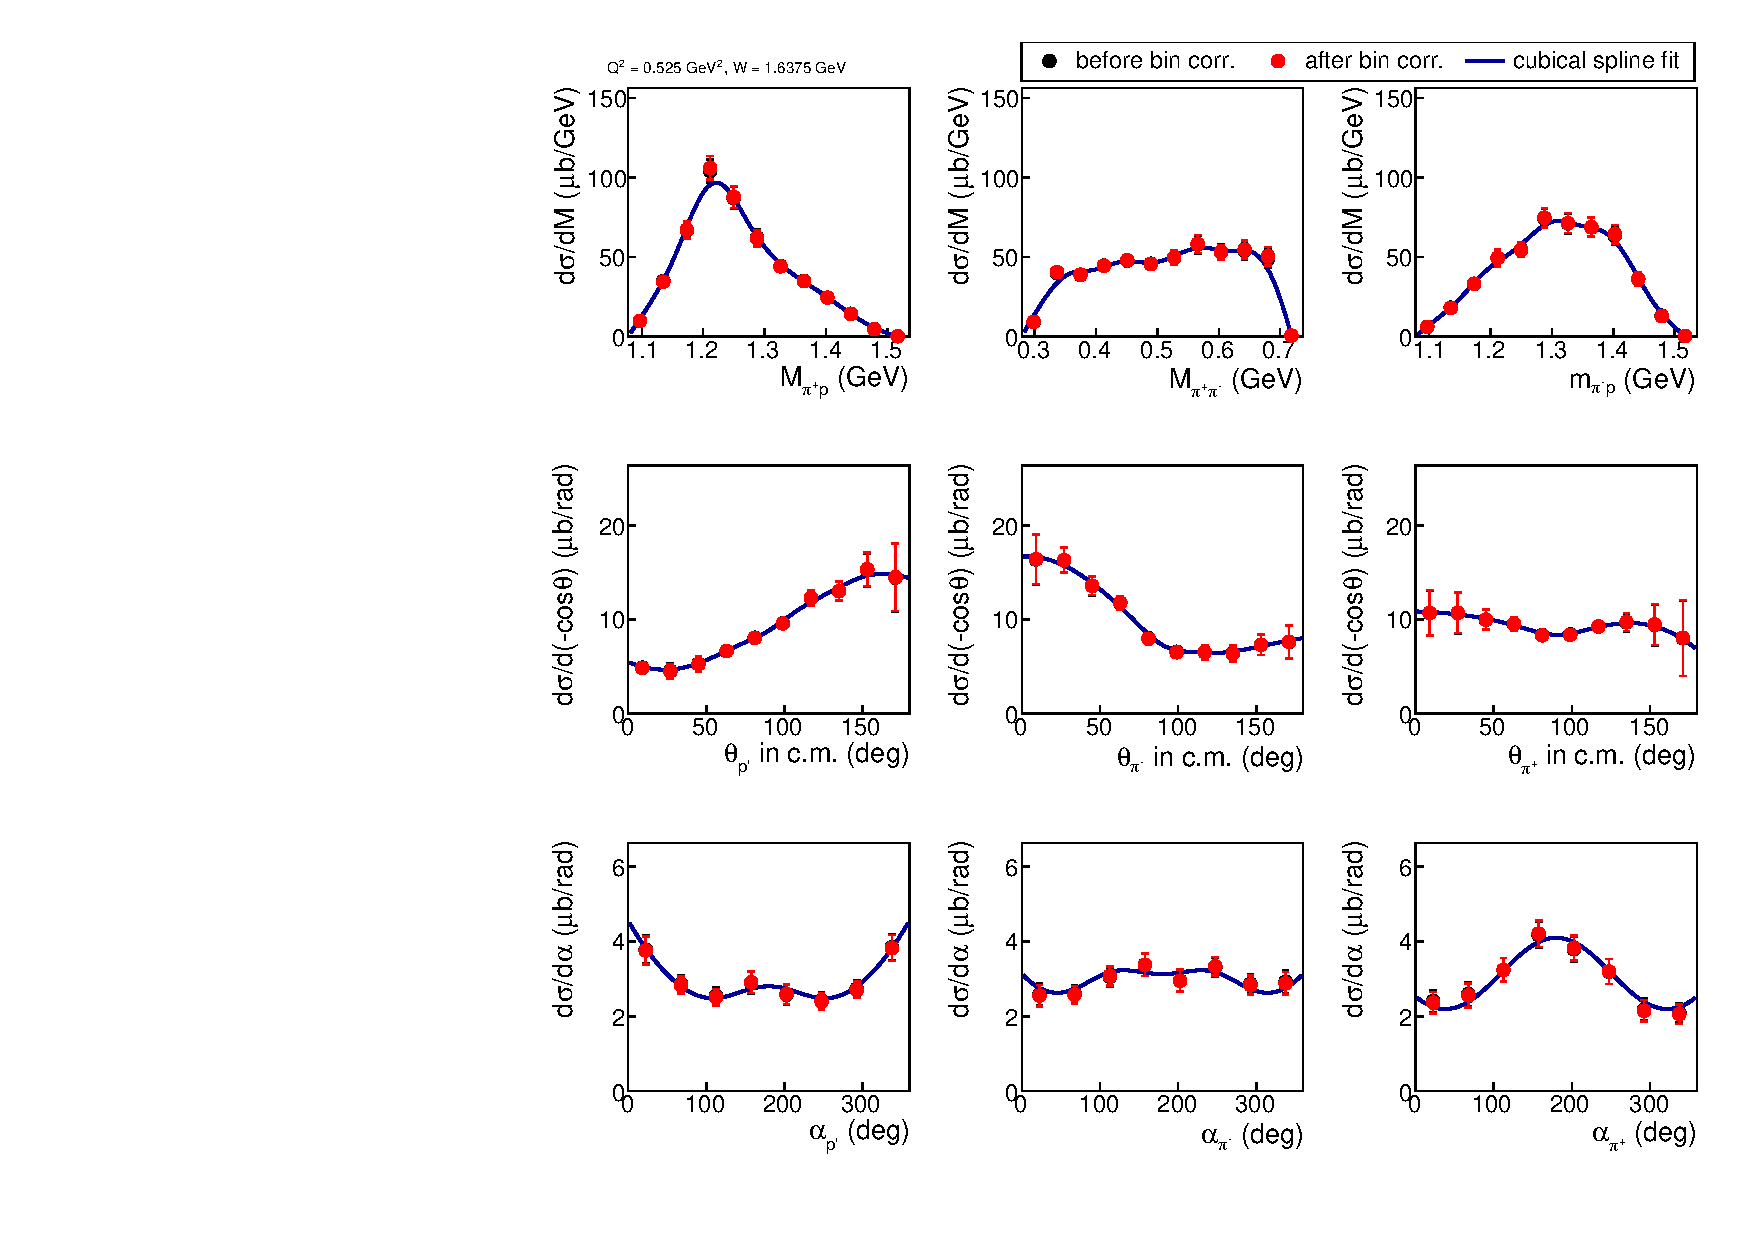
\includegraphics[width=13.5cm]{pictures/corrections/bin_cor_1d.pdf}}
\caption{\small Single-differential cross sections as functions of the final hadron variables before (black points) and after (red points) the binning corrections. Curves represent a cubic spline approximation. The example is given for a particular $\Delta W \Delta Q^{2}$ bin with the central point $W=1.6375$~GeV and $Q^{2}=0.525$~GeV$^{2}$.  } \label{fig:bin_cor_1d}
\end{center}
\end{figure}



The integral cross sections are subjected to individual corrections of the $Q^{2}$ dependence inside the $W$ bins and the $W$ dependence inside the $Q^{2}$ bins, as shown on the left and right plots of Fig.~\ref{fig:bincor_w_q2}, respectively. In this figure black and red points represent the cross section values before and after binning corrections, respectively, while the curves correspond to the continuous cross section approximation. The latter are based on a second order polynomial fit of the $Q^{2}$ distributions (left plot) and on a cubic spline approximation for the $W$ distributions (right plot). The splines are forced to pass through the intermediate points that are obtained by averaging over two neighboring cross section points. In this way, the integral cross section value in each $\Delta W\Delta Q^{2}$ bin acquires two multiplicative correction factors. The corrections obtained for the integral distributions are then propagated to the single-differential cross sections.

\begin{figure}[htp]
\begin{center}
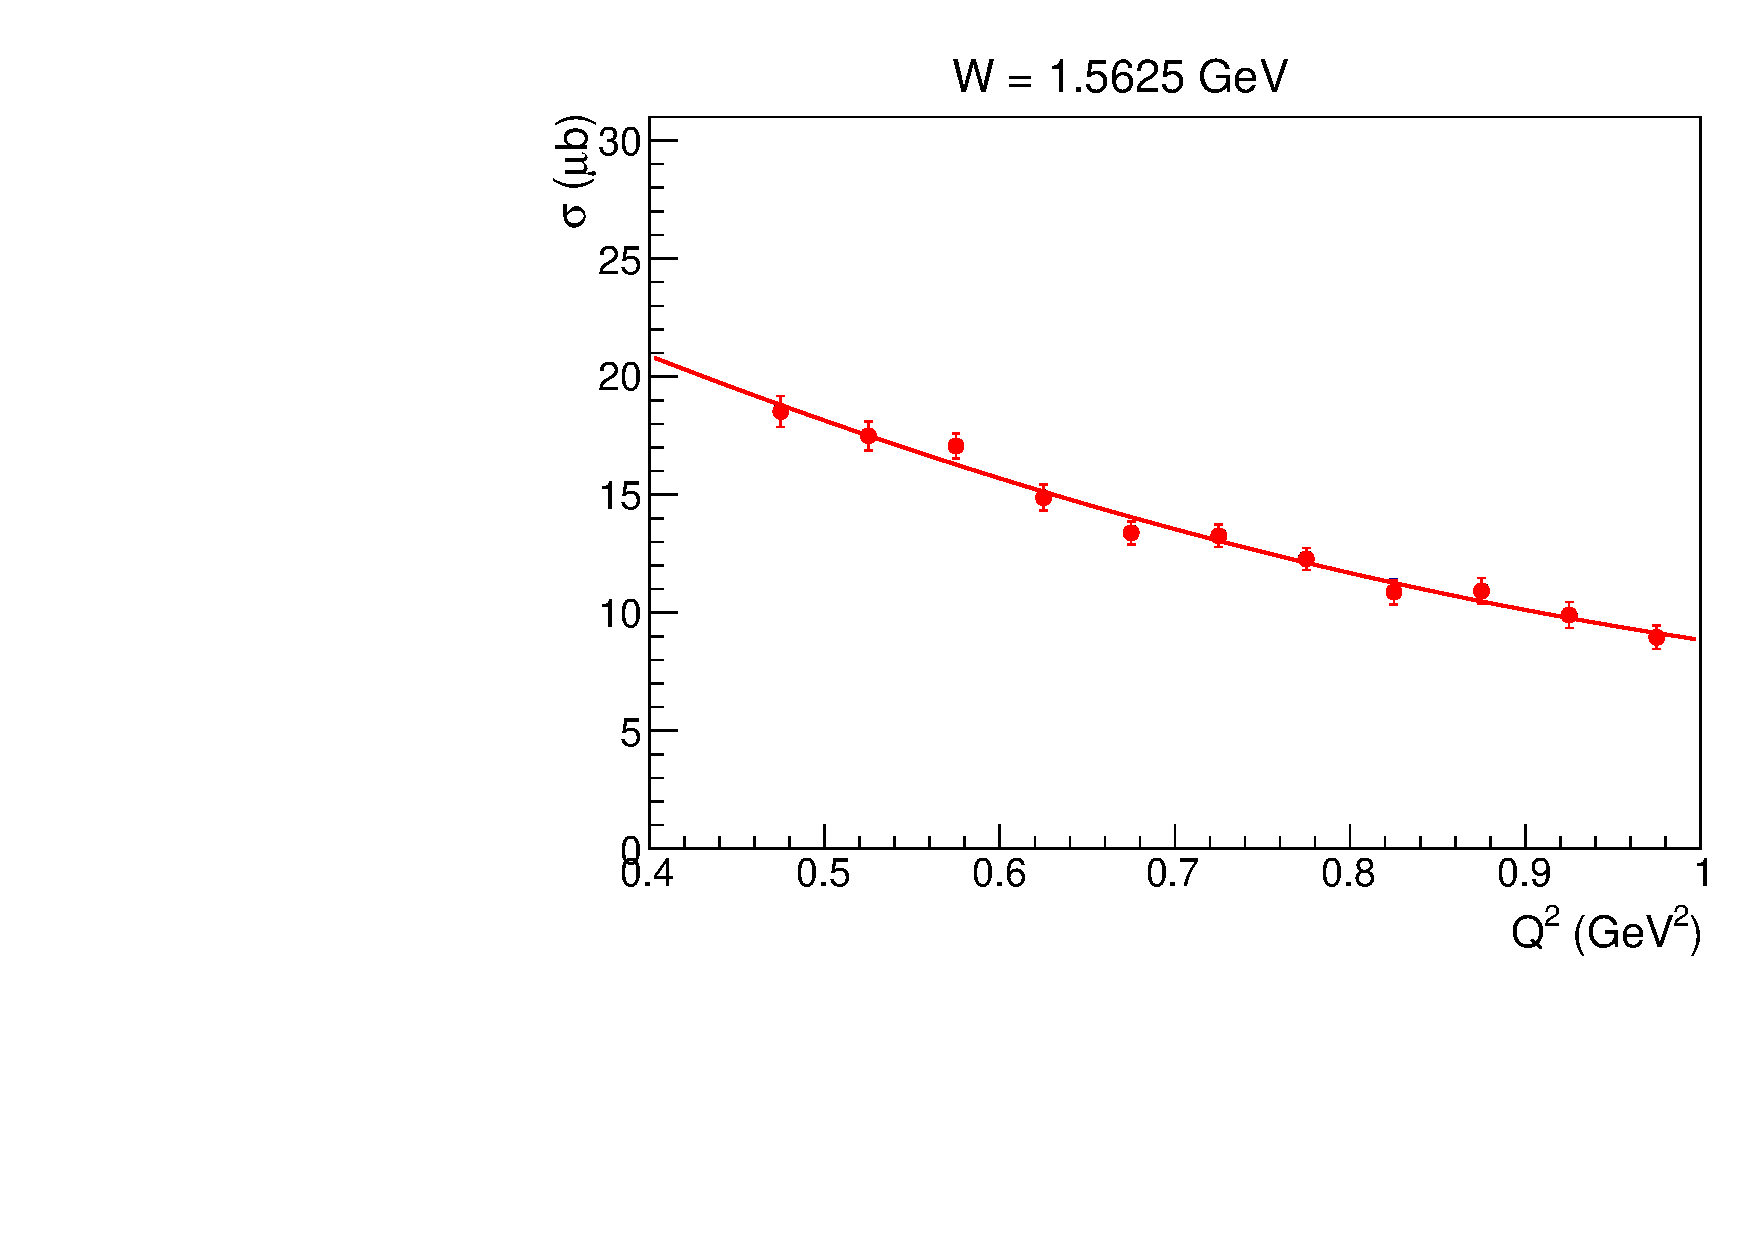
\includegraphics[width=8cm]{pictures/corrections/bin_cor_q2.pdf}
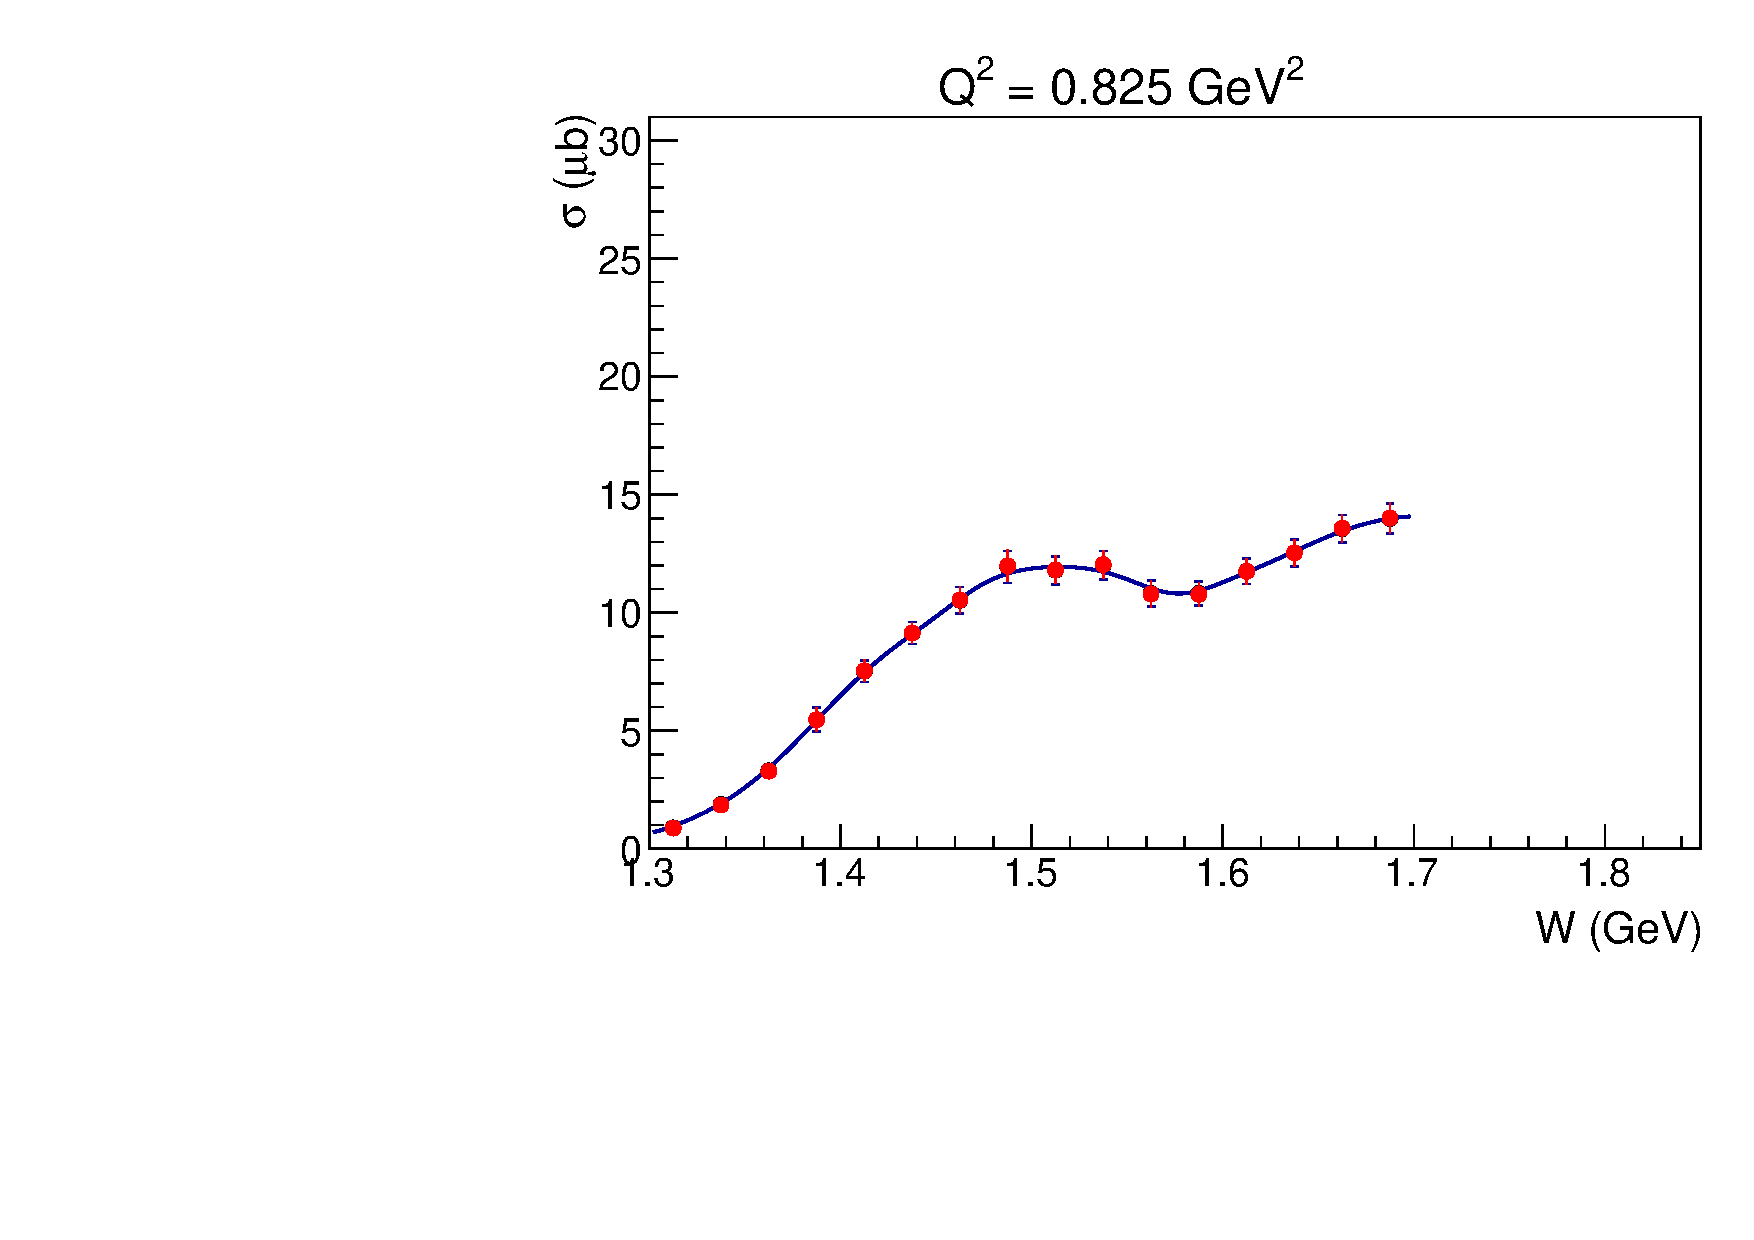
\includegraphics[width=8cm]{pictures/corrections/bin_cor_w.pdf}
\caption{\small $Q^{2}$ dependence (left plot) and the $W$ dependence (right plot) of the integral cross sections before (black points) and after (red points) the binning corrections. The curves correspond to a second order polynomial fit for the left plot and a cubic spline approximation for the right one. Each distribution is plotted for one particular bin as specified above the plots.} \label{fig:bincor_w_q2}
\end{center}
\end{figure}
 
Since in this analysis a relatively fine binning in all kinematic variables is chosen (see Sect.~\ref{Sect:binning}), the effect of the binning corrections is almost insignificant. 
This is why in Figs.~\ref{fig:bin_cor_1d} and~\ref{fig:bincor_w_q2} the black points (before the correction) are almost completely covered by the red ones (after the correction). For the $Q^{2}$ dependences the correction factors are less than 1\% in all bins, and for the $W$ dependences they are $\sim$2\%-3\% for the first two low $W$ bins and less than 1\% in all other bins. For the single-differential distributions, the corrections are on the level of 1\%-2\% for the majority of bins, but rise for some points (mostly at low $W$) up to 5\%-6\%.

